\section{Results} \label{sec:3}
The final results for the $v_{2}$ elliptic flow coefficient were obtained using the method in (\ref{subsec:2.2}) and was processed and visualized using the ROOT library.

\begin{figure}[h]
	\centering
	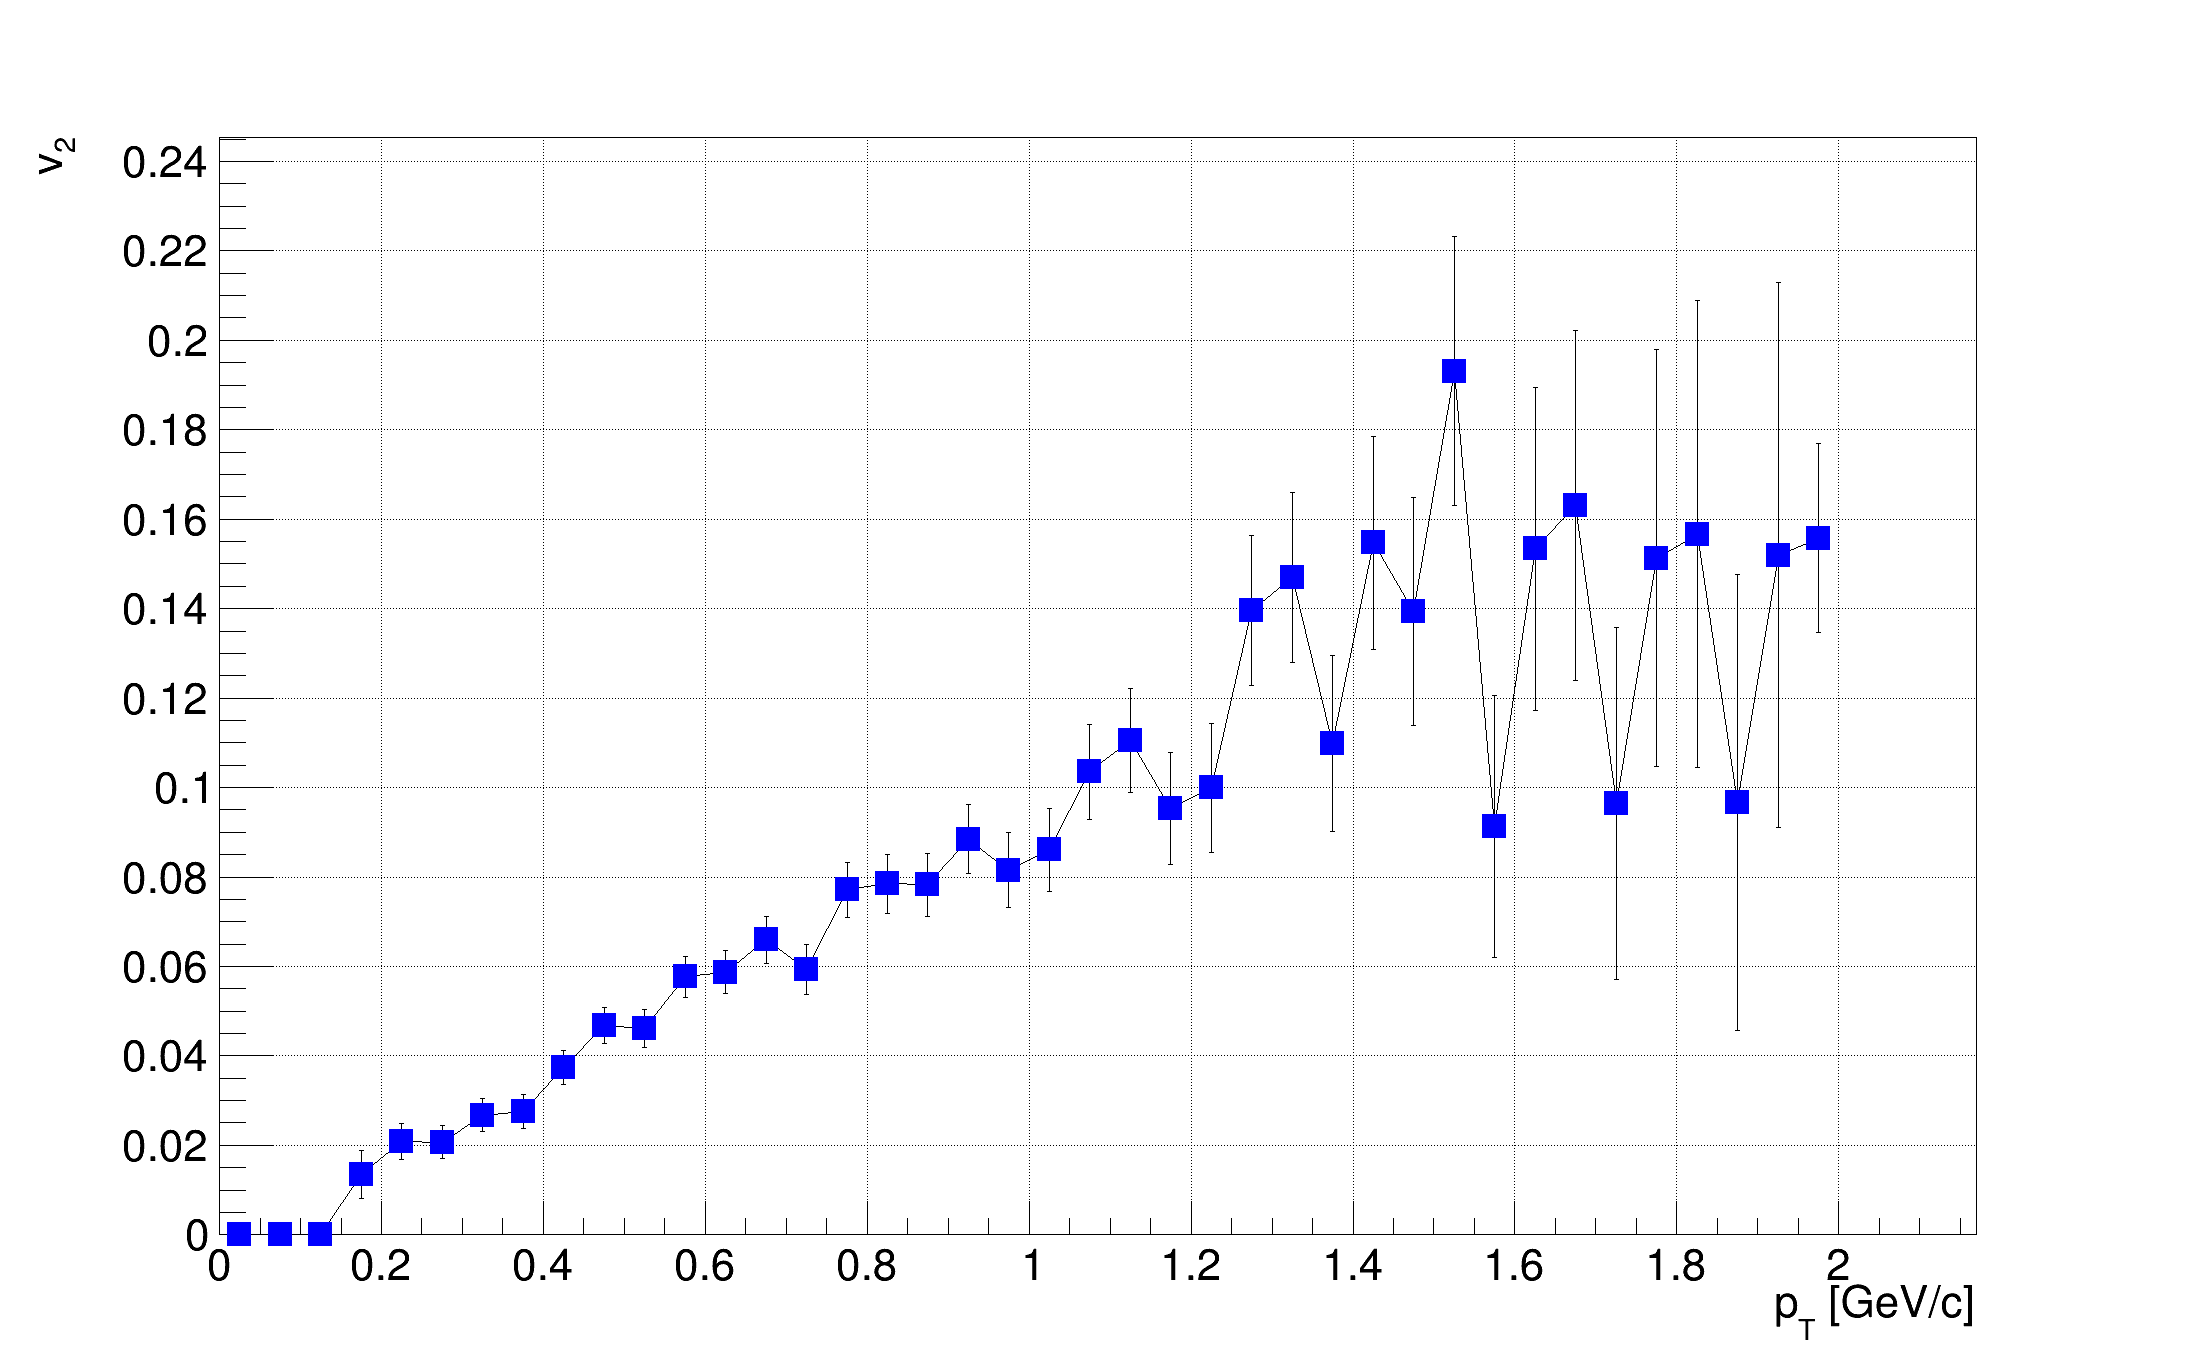
\includegraphics[width=\textwidth]{v2_flow_per_pt.png}
	\captionof{figure}{The $v_{2}$ elliptic flow coefficient as a function of the $p_{T}$ transverse momentum for a single centrality class of $0\% - 92\%$.}\label{fig:4}
\end{figure}

For this numerous literature can be cited eg. Fig. (2) in \citep{Collaboration2003} -- as it was already mentioned here. The very same characteristics can be observed the obtained results on Fig. (\ref{fig:3}) and in the cited article on Fig. (2). One can easily seen on both figures that the $p_{T} - v_{2}$ curve saturates as it reaches $p_{T} \approx 1$ or $2\ \mathrm{GeV}/\mathrm{c}$, just like as it is mentioned in eg. \citep{Collaboration2003} or \citep{Retiere2004}. The maximum value of $v_{2}$ is approximately $0.16$, but the large errors in the high $p_{T}$ regime makes it impossible to estimate it more precisely. Nonetheless this value also coincides with Fig. 2. in \citep{Collaboration2003}, where $v_{2} \left( p_{T} = 2\ \mathrm{GeV}/\mathrm{c} \right) \approx 0.16 - 0.17$.

At the end I've obtained results consistent with values in the literature, which implies that the calculations here were probably correct. The errors of the $v_{2}$ values could be probably improved by choosing a more robust fitting method for the angle distribution, but it probably won't change the final implications of the results.